% https://ask.latexstudio.net/ask/question/17406.html
\documentclass{article}
\usepackage{amsmath}
\usepackage{tikz}
\usetikzlibrary{matrix, calc}

\tikzset{%
    my matrix/.style={%
        matrix of math nodes,
        left delimiter=|,
        right delimiter=|,
        column sep=1.5em,
        row sep=1.5em,
        inner sep=0.3ex
    }%
}%

\begin{document}
\centering
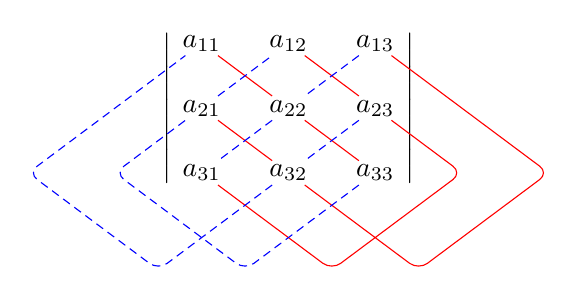
\begin{tikzpicture}
\matrix[my matrix] (M) {
a_{11} & a_{12} & a_{13} \\
a_{21} & a_{22} & a_{23} \\
a_{31} & a_{32} & a_{33} \\
};

\begin{scope}[draw=gray!70, rounded corners,
    x={($ (M-2-2) - (M-1-1) $)}, y={($ (M-2-1) - (M-1-2) $)}]
    \draw[red] 
    (M-1-1) -- (M-2-2) -- (M-3-3)
    (M-1-2) -- (M-2-3) -- ++(1,0) -- ++(0,1.5) -- (M-3-1)
    (M-1-3) -- ++(2,0) -- ++(0,1.5) -- (M-3-2) -- (M-2-1);
    \draw[densely dashed, blue]
    (M-1-3) -- (M-2-2) -- (M-3-1)
    (M-2-3) -- (M-3-2) -- ++(0,1.5) -- ++(-1.5,0) -- (M-1-1)
    (M-3-3) -- ++(0,1.5) -- ++(-1.5,0) -- (M-2-1) -- (M-1-2);
\end{scope}
\end{tikzpicture}
\end{document}
